\section{Empirical results}

\subsection{Evaluating HPS under covariate and model shifts}

\begin{figure}[!t]
	\begin{subfigure}[b]{0.33\textwidth}
		\centering
		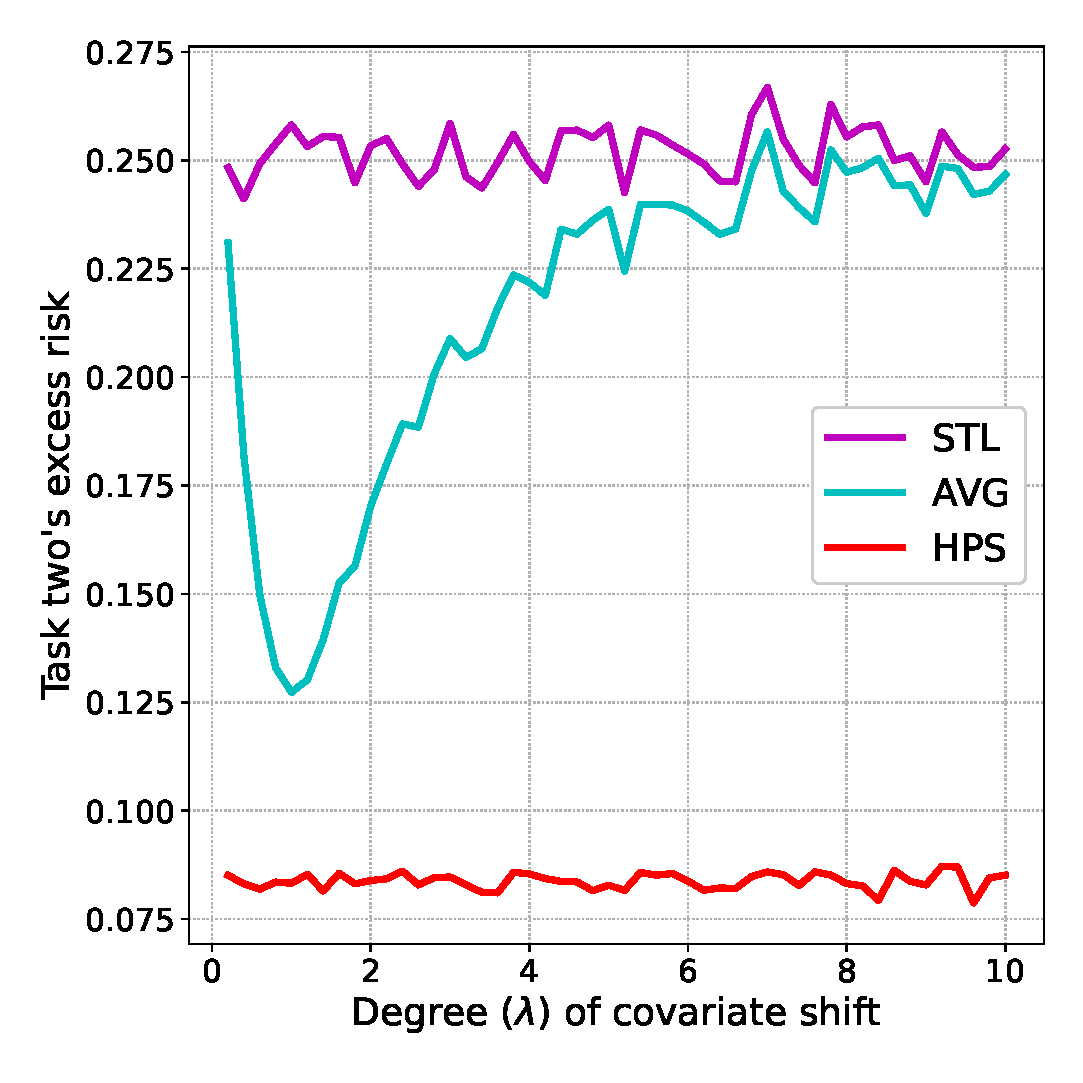
\includegraphics[width=0.95\textwidth]{figures/compare_risk_covariate_shift.eps}
		\caption{Covariate shift}
		\label{fig_sec5_covariate}
	\end{subfigure}\hfill%
	\begin{subfigure}[b]{0.33\textwidth}
		\centering
		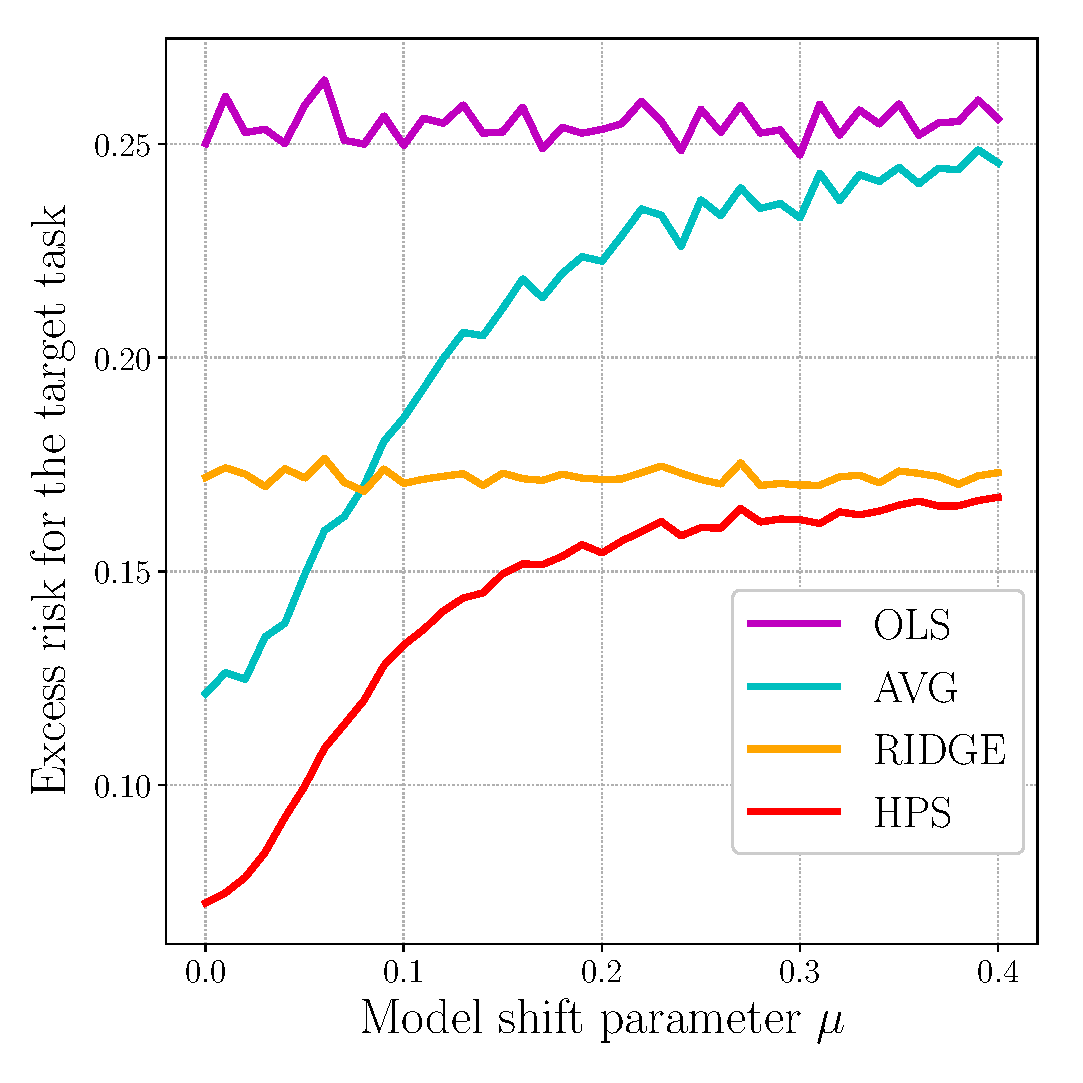
\includegraphics[width=0.95\textwidth]{figures/compare_risk_model_shift.eps}
		\caption{Model shift}
		\label{fig_sec5_model}
	\end{subfigure}\hfill%
	\begin{subfigure}[b]{0.33\textwidth}
		\centering
		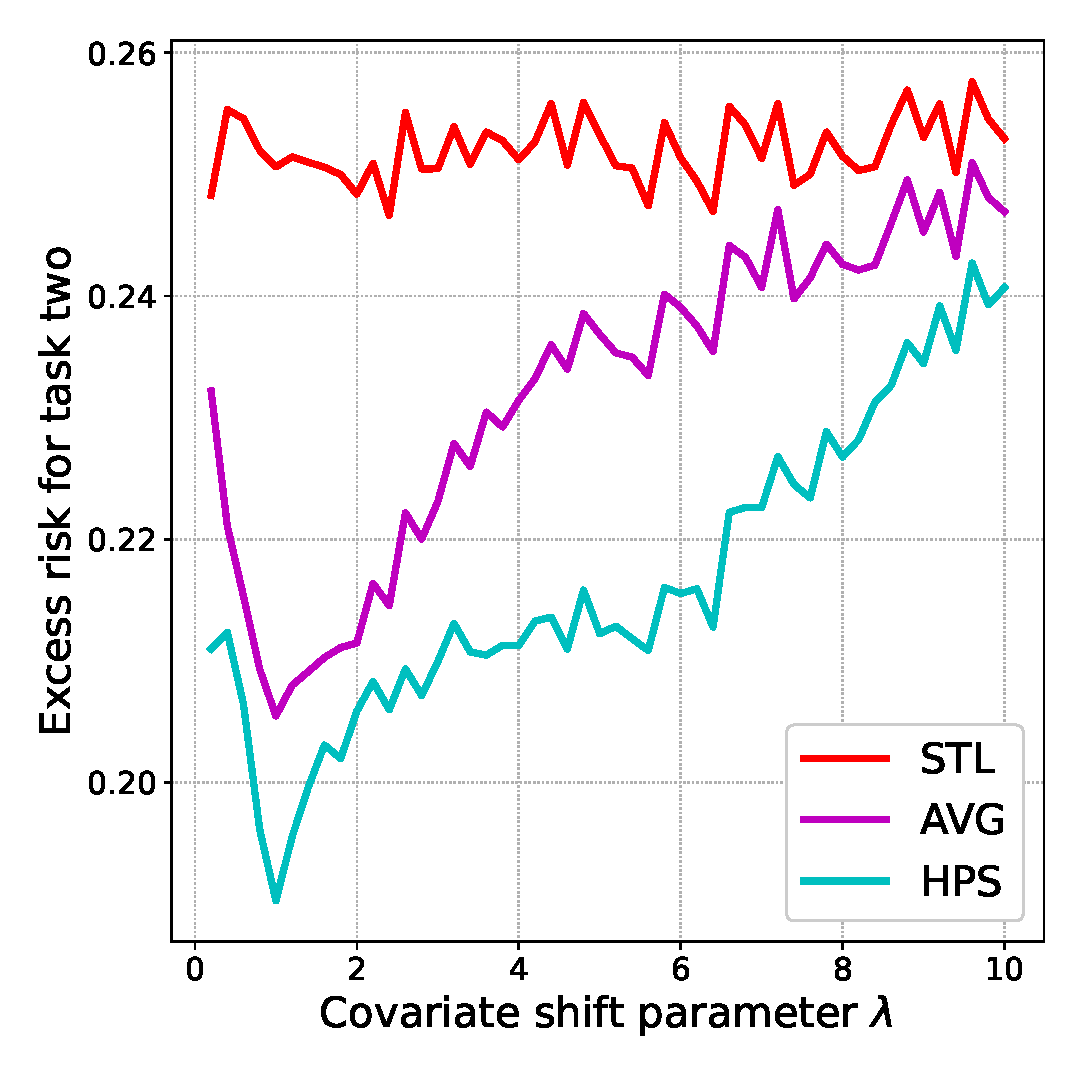
\includegraphics[width=0.95\textwidth]{figures/compare_risk_cov_model_shift.eps}
		\caption{Covariate and model shift}
		\label{fig_sec5_cov_model}
	\end{subfigure}
	\caption{We compare the empirical excess risk of HPS and several natural transfer learning estimators. We find that HPS achieves the lowest excess risk for predicting task two under (either or both) covariate and model shift. This simulation uses $p = 100, n_1 = n_2 = 200, \sigma = 1/2$. Figure \ref{fig_sec5_cov_model} uses $\lambda = 4$ for generating covariate-shifted data.}
	\label{fig_sec51}
\end{figure}

We show that HPS estimators enjoy superior empirical performance compared to several natural transfer learning estimators.
We consider the following estimators for this comparative study:
\begin{itemize}
    \item {\bf Averaging estimator (AVG):} given two tasks, take a convex combination of their OLS estimators $b \cdot \hat{\beta}^{\STL}_1 + (1 - b) \cdot \hat{\beta}^{\STL}_2$.
    \item {\bf STL estimator (STL):} simply use the OLS estimator of task two $\hat{\beta}^{\STL}_2$ without using task one's data.
    \item {\bf Transfer learning estimator (TL):} simply use the OLS estimator of task one $\hat{\beta}^{\STL}_1$ without using task two's data.
\end{itemize}
The parameter $b$ in the averaging estimator is optimized using a validation set of the same size as the training set.
Additionally, we extend the two-layer neural network formulation of HPS (cf. equation \eqref{eq_hps}) to a weighted objective:
$b \cdot \bignorm{X^{(1)} B A_1 - Y^{(1)}}^2 + (1 - b) \cdot  \bignorm{X^{2} B A_2 - Y^{(2)}}^2$, and optimize $b$ using the same validation set.

Figure \ref{fig_sec51} shows the result under (either or both) covariate and model shift.
Figure \ref{fig_sec5_covariate} uses the same data generating process as Figure \ref{fig_sec31}.
Figure \ref{fig_sec5_model} uses the same data generating process as Figure \ref{fig_sec3_model_shift}.
Figure \ref{fig_sec5_cov_model} further combines the covariate-shifted data and the model shift setting.
For reach run, we average the result over 100 random seeds because of high variance from using only a limited number of samples.
We find that HPS outperforms all the other estimators in this simulation (the result for the TL estimator is worse than STL and is omitted from the figure).

%\subsection{Implications for regression methods}


\subsection{Implications for neural networks}

\begin{wrapfigure}[12]{r}{0.3\textwidth}
	\vspace{-0.35in}
	\begin{center}
		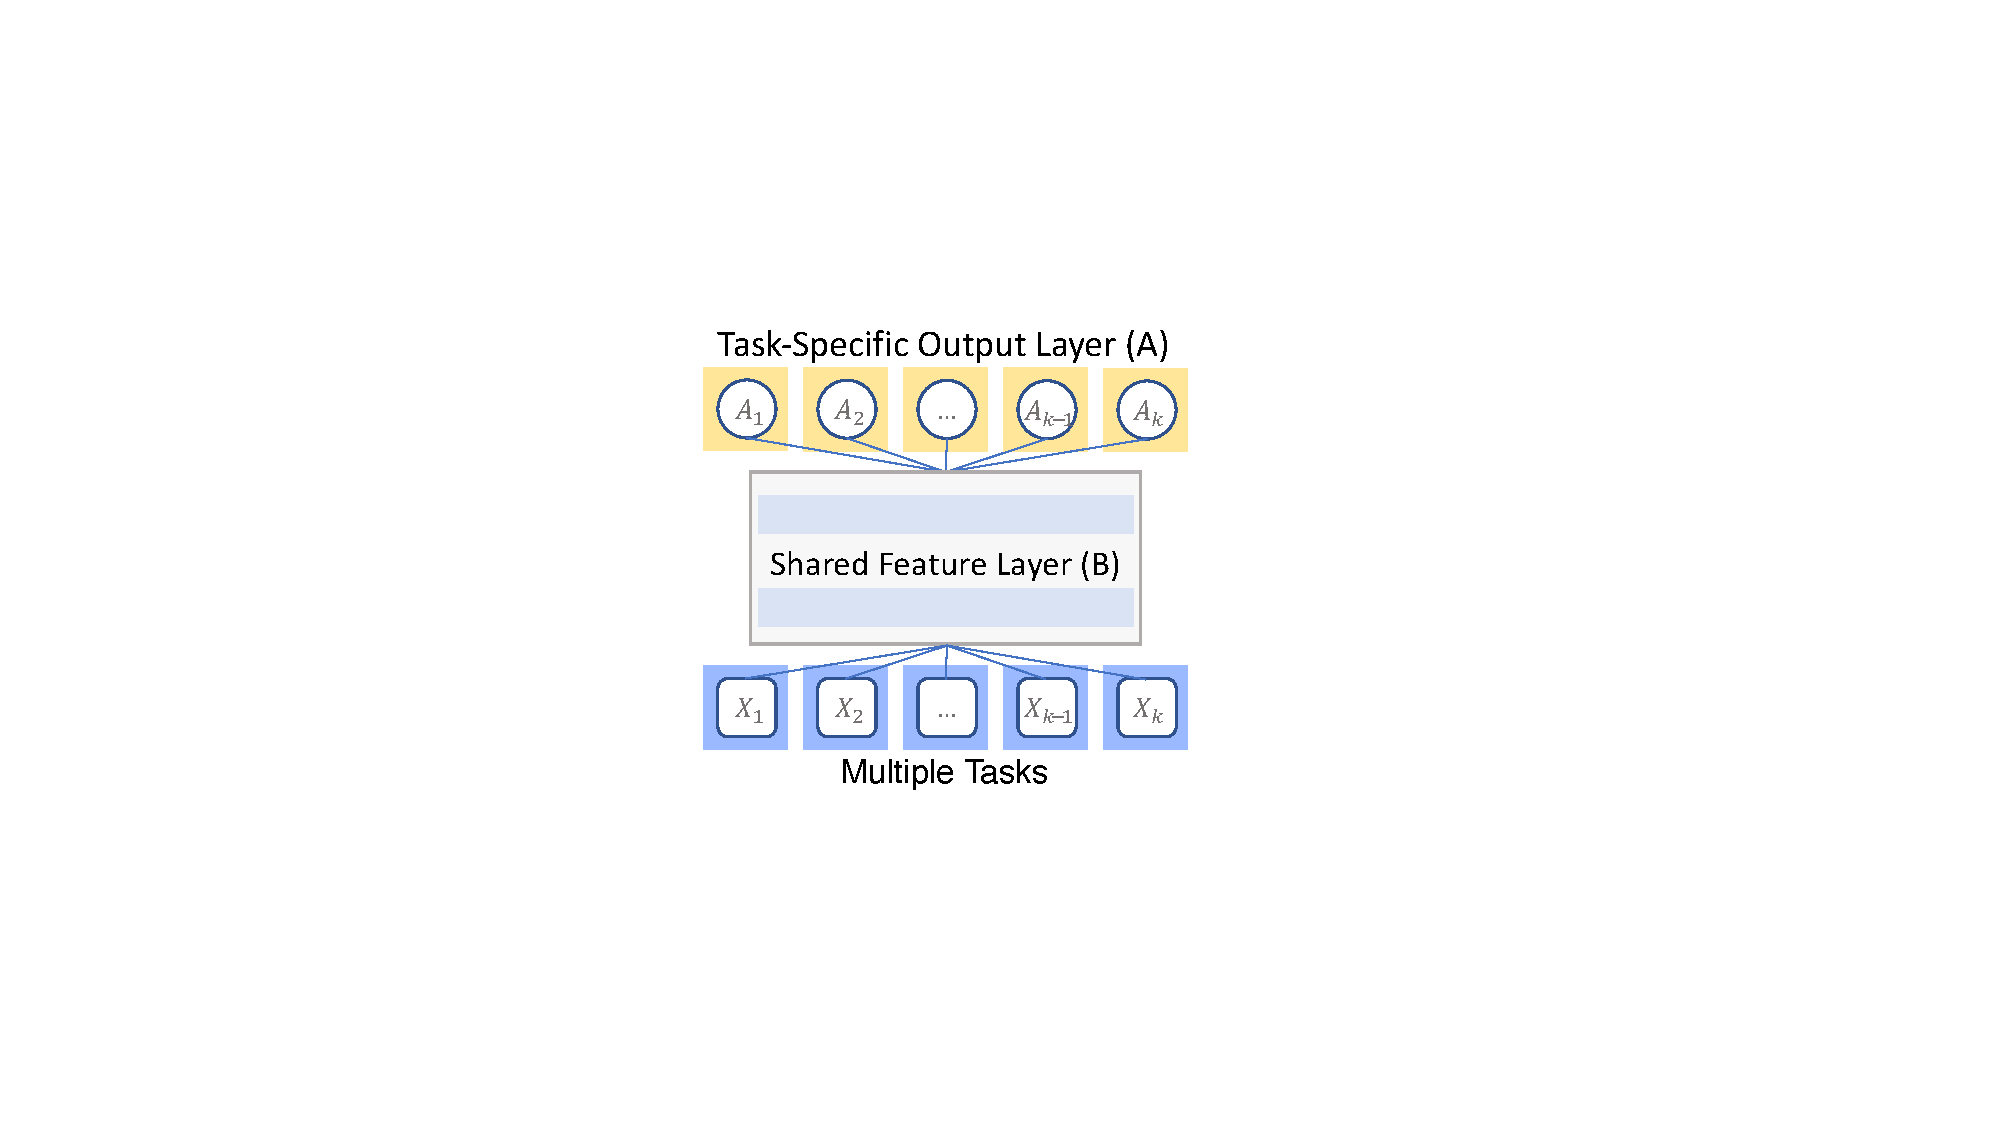
\includegraphics[width=0.27\textwidth]{figures/mtl_model_arch.pdf}
	\end{center}
	\vspace{-0.28in}
	\caption{A hard parameter sharing architecture.}
	\label{fig_intro_arch}
\end{wrapfigure}
We conduct further studies of HPS for text classification tasks.
We consider six datasets for predicting movie review sentiment (MR and SST) \cite{pang2005seeing,socher2013recursive}, sentence subjectivity (SUBJ) \cite{pang2004sentimental}, customer review sentiment (CR) \cite{hu2004mining}, question types (TREC) \cite{li2002learning}, and polarity of a phrase (MPQA) \cite{wiebe2005annotating}.\footnote{The datasets can be downloaded at \url{https://github.com/harvardnlp/sent-conv-torch/tree/master/data}. Further statistics of each dataset can also be found following the link.}
%The question is to predict positive or negative sentiment expressed in the text.
We learn a hard parameter sharing model that consists of a word embedding layer using GloVe \cite{pennington2014glove}, followed by a shared feature representation layer.\footnote{The GloVe word vectors can be downloaded at \url{https://nlp.stanford.edu/projects/glove/}.}
A separate output layer is used for predicting the labels of each dataset.
We evaluate on three possibilities of feature representation layers including LSTM, MLP, and CNN \cite{lei2018simple}.\footnote{Before the MLP layer, we apply an average pooling layer over the embedding of every word in the sentence.}
See Figure \ref{fig_intro_arch} for an illustration of the network architecture.

\paragraph{Covariate alignment for mitigating covariate shift.}
We apply our theoretical insights to conduct detailed analysis of a covariate alignment procedure proposed by \citet{WZR20}.
The idea of this procedure is to insert an ``alignment'' module (or matrix) between every input $X_i$ and the shared module $B$.
During training, the entire network is optimized together with this alignment module (see \citet{WZR20} for more details about the implementation).

Our hypothesis is that as $n_1 / n_2$ increases, performing covariate alignment leads to larger accuracy improvement over the baseline HPS.
Recall from Claim \ref{prop_covariate} that covariate shift between the data source and the target task worsens the performance of HPS.
The effect is further exacerbated when the sample size of the data source is larger than the target task.
%This observation highlights the need for mitigating covariate shift when $n_1 / n_2$ increases.
To verify the hypothesis, we conduct multi-task training over all 15 pairwise tasks (among the six datasets).
We measure the average accuracy improvement from performing covariance alignment vs. HPS (trained using stochastic gradient descent (SGD)) over the 15 task pairs.
Figure \ref{fig_ab_cov} confirms our hypothesis.
We observe that covariate alignment achieves up to 4\% accuracy improvement as $n_1 / n_2$ increases.
%We fix task two's sample size at $1,000$, and increase task one's sample size from $1,000$ to $3,000$.

\begin{figure}[!t]
	\begin{subfigure}[t]{0.5\textwidth}
		\centering
		\vspace{0pt}
		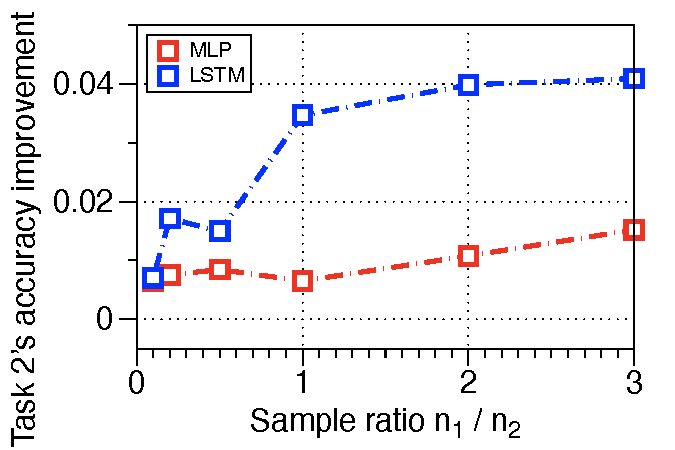
\includegraphics[width=0.8\textwidth]{figures/fig3b.pdf}
		\caption{Covariate alignment under varying sample sizes}
		\label{fig_ab_cov}
	\end{subfigure}\hfill
	\begin{subfigure}[t]{0.5\textwidth}
		\centering
		\vspace{0pt}
		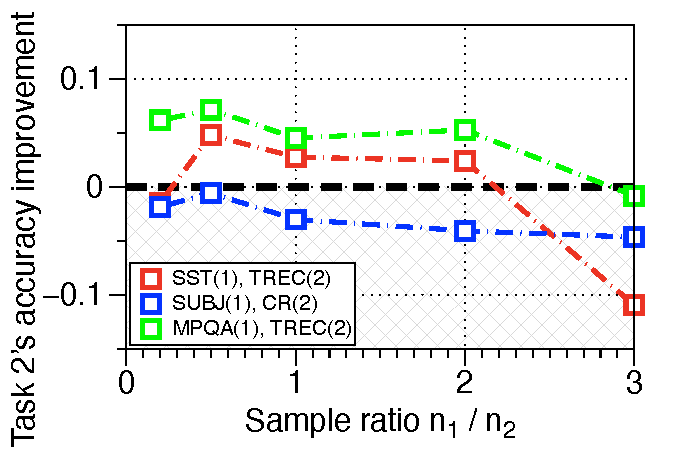
\includegraphics[width=0.8\textwidth]{figures/fig3a.pdf}
		\caption{Information transfer under varying sample sizes}
		\label{fig_ab_data}
	\end{subfigure}
	\caption{Comparing hard parameter sharing (HPS) to single-task learning (STL) and a covariate alignment approach proposed by \cite{WZR20}:
	In Figure \ref{fig_ab_data}, we observe that for multiple task pairs, increasing task one's sample size improves task two's prediction accuracy initially, but hurts eventually -- a phenomenon similar  to Figure \ref{fig_size}.
	This experiment fixes $n_2 = 1000$ while varying $n_1$.
	In Figure \ref{fig_ab_cov}, we observe that as task one's sample size increases, covariance alignment improves more over HPS.
	On the $y$-axis, we plot task two's test accuracy using HPS, subtracted by its STL test accuracy.
    We fix task two's sample size at $1000$ and increase task one's sample size from $100$ to $3000$.}
	\label{fig_text}
\end{figure}

%For the text classification experiment, we encode each word using the GLoVe word embeddings.%
%\textit{Predicting transfer effect via STL results.}
%We show that the single-task based metric proposed in Section \ref{sec_similarity} can predict positive or negative transfer in MTL.
%A common challenge in the study of MTL is that the results can be hard to understand.
%It is difficult to predict when MTL performs well without running extensive trials.
%Our insight is that we can use STL results to help understand MTL results.
%Table \ref{tab:mtl_better_than_stl} shows the result on both the sentiment analysis and the ChestX-ray14 tasks.
%We find that using a threshold of $\tau = 0.1$, the STL results correctly predict positive or negative transfer with $75.6\%$ precision and $38.8\%$ recall among $30$ times $5$ (random seeds) task pairs!
%We observe similar results for $91$ task pairs from the ChestX-ray14 dataset.
%The results show that STL results are indicative of MTL results.

\paragraph{Progressive training for mitigating model shift.}
Inspired by our theoretical analysis, we propose a progressive training procedure that reduces the computational cost of learning HPS networks.
To motivate this procedure, we first conduct an experiment similar to Figure \ref{fig_sec3_model_transition}) but using the text classification datasets instead.
In Figure \ref{fig_ab_data}, we find that for multiple pairs of datasets, increasing $n_1$ improves task two's test accuracy initially, but hurts eventually.

These examples and the ones in Figure \ref{fig_sec3_model_transition} suggest a natural progressive training procedure that increases $n_1$ progressively until performance drops.
Concretely, we first divide the training data into $S$ batches.
Then, we progress in $S$ stages during training. During each stage, we progressively add one more minibatch of data from the data source(s).
During each stage, we run SGD for $T$ epochs using only the available minibatches of data.
We terminate once task two's validation accuracy drops compared to the previous round's result or reaches a desired threshold $\tau$.
See Algorithm \ref{alg_inc_train} for the complete procedure.
As an example, this procedure will terminate at the optimal value of $n_1$ if applied to the settings of Figures  \ref{fig_sec3_model_transition} and \ref{fig_ab_data}.
In light of these observations, our hypothesis is that this procedure requires a lower computational cost compared to SGD.
%For example, if the procedure terminates at 30\% of all batches, then SGD only passes over 30\% of its data, whereas standard round-robin training passes over 100\% of task one's data.

\begin{algorithm}[!h]
	\caption{Progressive training of hard parameter sharing networks}
	\label{alg_inc_train}
	\begin{algorithmic}[1]
		\Input Two tasks $(X^{(1)}, Y^{(1)})$ and $(X^{(2)}, Y^{(2)})$.
		\Param A shared module $B$, and output layers $A_1, A_2$.
		\Req Number of batches $S$, epochs $T$, task $2$'s validation accuracy $\hat{g}(B; A_2)$, a threshold $\tau\in(0,1)$.
		\Output The trained modules $B, A_2$ optimized for task $2$.
		\State Divide $(X^{(1)}, Y^{(1)})$ randomly into $S$ batches: $(x^{(1)}, y^{(1)}), \dots, (x^{(S)}, y^{(S)})$.
		\For{$i = 1,\dots, S$}
		\For{$j = 1,\dots, T$}
		\State Minimize the cross-entropy loss of $B, A_1, A_2$ on $\set{x^{(k)}, x^{(k)}}_{k=1}^i$ and  $(X^{(2)}, Y^{(2)})$ using SGD.
		\EndFor
		\State Let $a_i = \hat{g}(B; A_2)$ be the validation accuracy.
		\If{$a_i < a_{i-1}$ or $a_i > \tau$}
		\State \textbf{break}
		\EndIf
		\EndFor
	\end{algorithmic}
\end{algorithm}


\begin{wrapfigure}[9]{r}{0.3\textwidth}
	\vspace{0.0in}
	\centering
	\begin{tabular}{c c c}
		\toprule
		Models & Relative cost \\
		\midrule
		{\bf CNN}  & 30\% \\
		{\bf LSTM} & 35\% \\
		{\bf MLP}  & 31\%  \\
		\bottomrule
		\end{tabular}
		\captionof{table}{The computational cost of running Algorithm \ref{alg_inc_train} relative to the cost of running SGD.}
		\label{tab:taskonomy}
	\label{fig_intro_arch}
\end{wrapfigure}
We evaluate Algorithm \ref{alg_inc_train} under two scenarios.
First, we consider all $15$ pairwise tasks and use the first task as a data source to help predict the second task.
We find that when averaged over all $15$ two-task pairs, our procedure requires less than $35\%$ of the computational cost relative to SGD while reaching the same level of test accuracy for predicting task two.
%Our insight is that since adding more samples from the source task does not always help, we can improve efficiency by adding source samples \textit{progressively} during training.
%\textbf{Improving transfer learning training efficiency.}
%We show that Algorithm \ref{alg_inc_train} also applies to transfer learning settings.
%Compared to fine-tuning the source model on the target task, we show that our proposed method reduces the computional cost by \alert{$xx\%$}, without sacrificing accuracy.
Second, we consider using all six datasets as data sources to help predict every other task---that is, we measure the average accuracy of predicting all six tasks.
We find that a similar progressive training style procedure requires less than $35\%$ of the computational cost for reaching the same average test accuracy compared to SGD.

\medskip
\noindent\textit{Further details.} We task two's test accuracy and set $\tau$ as task two's test accuracy obtained via the standard round-robin training schedule.
We include all of task two's data and progressively add task one's data using the procedure described above.
Since the prediction accuracy has been controlled the same, we compare the computational cost.
We set $\tau$ to be the average test accuracy of all six tasks obtained using standard round-robin training.
We extend our procedure to all six datasets. We include the data from all tasks except SST. For SST, we progressively add data similar to the above procedure.



%\begin{figure}[!t]
%	\centering
%	\begin{subfigure}[b]{0.5\textwidth}
%		\centering
%		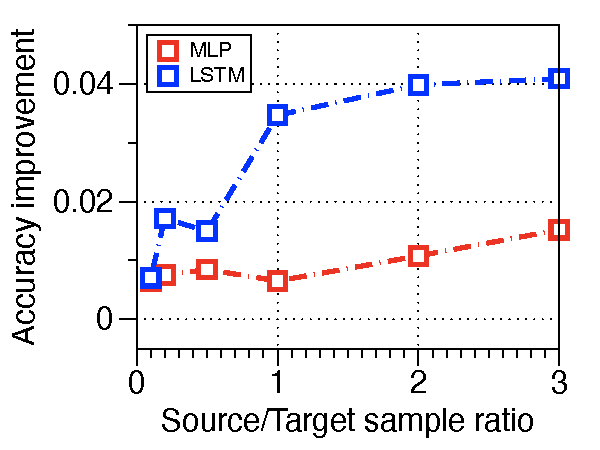
\includegraphics[width=0.5\textwidth]{figures/ratio_alignment_norm_diff_all.pdf}
%		\caption{Averaged over all 16 task pairs}
%		\label{fig_ab_cov}
%	\end{subfigure}\hfill
%	\begin{subfigure}[b]{0.5\textwidth}
%		\centering
%		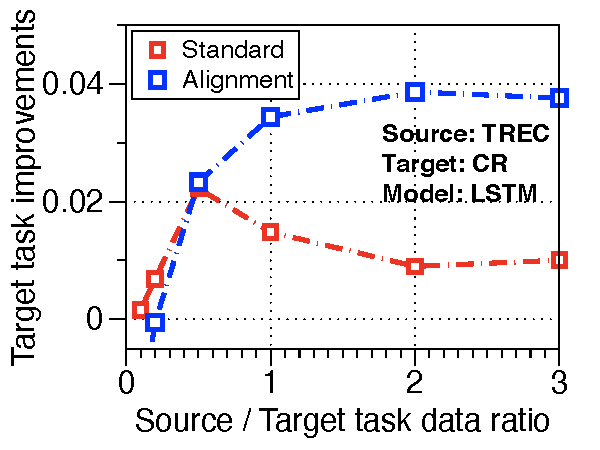
\includegraphics[width=0.5\textwidth]{figures/ratio_alignment_norm_trec_cr_lstm.pdf}
%		\caption{An example task pair}
%		\label{fig_cov_a}
%	\end{subfigure}
%	\caption{ (TREC and CR)}
%\end{figure}

%\textbf{Further results of the covariance alignment procedure.}
%Our results in Figure \ref{fig_ab_cov} are averaged over all the task pairs.
%In Figure \ref{fig_covariate_app}, we show two task pairs as examples.
%In Figure \ref{fig_cov_a}, we observe that for the particular task pair, covariance alignment provides more significant gains when the sample ratio is large.
%In Figure \ref{fig_cov_b}, we observe that covariance alignment does not always improve over the baseline multi-task learning model.
%One explanation is that MR and SST are similar tasks, hence adding the alignment module is unnecessary.
%An interesting question is to understand when adding the alignment module benefits the multi-task learning model.
%We leave this question for future work.
%Note: For text classification tasks, the source task training data size ranges from 500 to 1,500 and target task training data size is 1000; For ChestX-ray14,

%\begin{figure}[!h]
%	\centering
%	\begin{subfigure}[b]{0.48\textwidth}
%		\centering
%		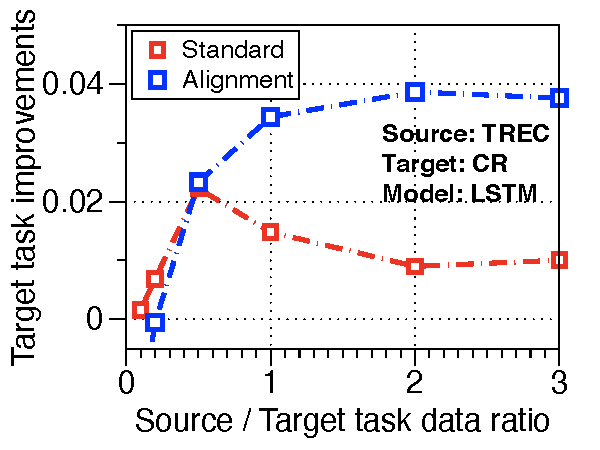
\includegraphics[width=0.7\textwidth]{figures/ratio_alignment_norm_trec_cr_lstm.pdf}
%		\caption{Task pair TREC and CR}
%		\label{fig_cov_a}
%	\end{subfigure}\hfill
%		\begin{subfigure}[b]{0.48\textwidth}
%		\centering
%		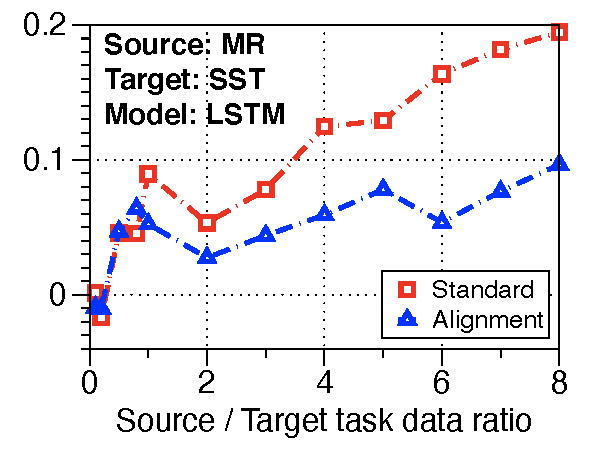
\includegraphics[width=0.7\textwidth]{figures/ratio_alignment_mr_sst_lstm.pdf}
%		\caption{Task pair MR and SST}
%			\label{fig_cov_b}
%	\end{subfigure}
%	\caption{(a) For the task pair TREC and CR, adding the covariance alignment procedure provides more improvement when the source/target sample ratio is large.
%	(b) For the task pair MR and SST, adding the covariance alignment procedure hurts performance.
%	One explanation is that MR and SST are similar tasks, hence adding the alignment module is unnecessary.}
%	\label{fig_covariate_app}
%\end{figure}